\documentclass[answers]{exam}
\usepackage{../../template}
\author{niceguy}
\title{Problem Set 1}
\begin{document}
\maketitle

\begin{questions}

\question{Write down the Schr\"odinger equation for a free particle, subject to no forces and hence with $U(\vec{r}) = 0$ everywhere, and show that the function $\psi(\vec{r}) = e^{i\vec{k}\cdot\vec{r}}$ is a solution for any fixed vector $\vec{k}$ satisfying $E = \frac{\hbar^2k^2}{2M}$. Can you suggest an interpretation for the vector $\hat{k}$?}

\begin{solution}
	$$\frac{\partial^2\psi}{\partial x^2} + \frac{\partial^2\psi}{\partial y^2} + \frac{\partial^2\psi}{\partial z^2} = -\frac{2ME}{\hbar^2}\psi$$
	Note that
	$$\frac{\partial \psi}{\partial x} = i(\vec{k}\cdot\vec{r}_x)\psi = i(\vec{k}\cdot\hat{i})\psi = ik_x\psi$$
	Hence substituting the given $\phi$ yields
	\begin{align*}
		\text{LHS} &= (-k_x^2 + -k_y^2 + -k_z^2)\psi \\
			   &= -k^2\psi \\
		\text{RHS} &= -\frac{\hbar^2k^2}{2M}\times\frac{2M}{\hbar^2}\psi \\
			   &= -k^2\psi \\
			   &= \text{LHS}
	\end{align*}

\end{solution}

\question{A mountain can be described by the function $h(x,y)$, which gives the height above sea level of a point that is $x$ east and $y$ north of the origin $O$.}

\begin{parts}
	\part{Describe in words the meaning of $\frac{\partial h}{\partial x}$ and $\frac{\partial h}{\partial y}$.}
	\part{What does it mean to a hiker who is walking due north if $\frac{\partial h}{\partial y}$ is positive?}
	\part{What if he is walking due north, but $\frac{\partial h}{\partial y}$ is 0 and $\frac{\partial h}{\partial x}$ is positive?}
\end{parts}

\begin{solution}
	The partial derivatives are the slopes at point $(x,y)$ along the $x$ and $y$ axes respectively.\\
	To the hiker, it means the slope is positive at his location along his path. \\
	The slope is (at least) momentarily 0 in the path he is walking along, but there is a non zero slope in the normal direction, from top right to bottom left.
\end{solution}

\question{Consider a particle of mass $M$ in a two-dimensional, rigid rectangular box with sides $a$ and $b$. Using the method of separation of variables, find the allowed energies and wave functions for this particle. In particular, show that the allowed energies are identified by two integers $n_x$ and $N_y$ and have the form
	$$E_{n_x,n_y} = \frac{\hbar^2\pi^2}{2M}\left(\frac{n^2_x}{a^2} + \frac{n^2_y}{b^2}\right)$$
} \label{this}

\begin{solution}
	Assume the energy component can be split into $x$ and $y$ components, i.e. $E = E_x + E_y$. Then
	$$\frac{\partial^2\psi}{\partial x^2} = -\frac{2ME}{\hbar^2}\psi$$
	and a similar equation exists for $y$. This can be solved the same way as the one dimensional case, yielding
	$$E_x = \frac{\hbar^2\pi^2n^2}{2Ma^2}$$
	and a similar equation for $y$. Summing yields
	$$E = E_x + E_y = \frac{\hbar^2\pi^2}{2M}\left(\frac{n^2_x}{a^2} + \frac{n^2_y}{b^2}\right)$$
\end{solution}

\question{Consider a particle in a rigid rectangular box with sides $a$ and $b = \frac{a}{2}$. Using the above result, find the lowest six energy levels with their quantum numbers and degeneracies.}

\begin{solution}
	Substituting yields
	$$E_{n_x,n_y} = \frac{\hbar^2\pi^2}{2Ma^2}(n^2_x + 4n^2_y)$$
	Then letting $k = \frac{\hbar^2\pi^2}{2Ma^2}$, we have
	\begin{center}
	\begin{tabular}{|c|c||c|}
		\hline
		$n_x$ & $n_y$ & Energy in terms of $k$ \\
		\hline\hline
		1 & 1 & 5 \\
		\hline
		2 & 1 & 8 \\
		\hline
		3 & 1 & 13 \\
		\hline
		1 & 2 & 17 \\
		\hline
		4 & 1 & 20 \\
		\hline
		2 & 2 & 20 \\
		\hline
		3 & 2 & 25 \\
		\hline
	\end{tabular}
	\end{center}
	where the degenerate energy level is 20$k$.
\end{solution}

\question{The energy levels of a particle in a cubical box can be found from the next question by setting $a=b=c$. Find the lowest eight energy levels for a particle in a three-dimensional, rigid cubical box. Draw an energy-level diagram for these levels, showing their quantum numbers, energies, and degeneracies.}

\begin{solution}
	Substituting yields
	$$E = \frac{\hbar^2\pi^2}{2Ma^2}(n^2_x + n^2_y + n^2_z)$$
	Similarly,
	\begin{center}
	\begin{tabular}{|c|c|c||c|}
	\hline
	$n_x$ & $n_y$ & $n_z$ & Energy in terms of $k$ \\
	\hline\hline
	1 & 1 & 1 & 3 \\
	\hline
	2 & 1 & 1 & 6 \\
	\hline
	1 & 2 & 1 & 6 \\
	\hline
	1 & 1 & 2 & 6 \\
	\hline
	2 & 2 & 1 & 9 \\
	\hline
	2 & 1 & 2 & 9 \\
	\hline
	1 & 2 & 2 & 9 \\
	\hline
	3 & 1 & 1 & 11 \\
	\hline
	1 & 3 & 1 & 11 \\
	\hline
	1 & 1 & 3 & 11 \\
	\hline
	2 & 2 & 2 & 12 \\
	\hline
	3 & 2 & 1 & 14 \\
	\hline
	3 & 1 & 2 & 14 \\
	\hline
	2 & 3 & 1 & 14 \\
	\hline
	2 & 1 & 3 & 14 \\
	\hline
	1 & 3 & 2 & 14 \\
	\hline
	1 & 2 & 3 & 14 \\
	\hline
	3 & 2 & 2 & 17 \\
	\hline
	2 & 3 & 2 & 17 \\
	\hline
	2 & 2 & 3 & 17 \\
	\hline
	4 & 1 & 1 & 18 \\
	\hline
	1 & 4 & 1 & 18 \\
	\hline
	1 & 1 & 4 & 18 \\
	\hline
	\end{tabular}
	\end{center}
	where the degenerate energy states are $6k, 9k, 11k, 14k, 17k, 18k$
\end{solution}

\question{Show that the allowed energies of a mass $M$ confined in a three-dimensional rectangular rigid box with sides $a, b, c$ are
	$$E = \frac{\hbar^2\pi^2}{2M}\left(\frac{n^2_x}{a^2} + \frac{n^2_y}{b^2} + \frac{n^2_z}{c^2}\right)$$
}

\begin{solution}
	Basically \ref{this}.
\end{solution}

\question{}
\begin{parts}
	\part{For the two-dimensional polar coordinates, prove the relation
		$$x = r\cos\phi \text{ and } y = r\sin\phi$$
	}
	\part{Find corresponding expressions for $r$ and $\phi$ in terms of $x$ and $y$.}
\end{parts}

\begin{solution}
	The first part involves a graphical proof and is trivial.
	$$r = \sqrt{x^2 + y^2}$$
	$$\phi = \arctan\left(\frac{y}{x}\right)$$
\end{solution}

\question{A certain point $P$ in two dimensions has rectangular coordinates $(x,y)$ and polar coordinates $(r,\phi)$. What are the polar coordinates of the point $Q(-x,-y)$?}

\begin{solution}
	$(r, \phi+\pi)$
\end{solution}

\question{A crucial step in solving the Schr\"odinger equation for the central force problem was the identity
	$$\frac{\partial^2\psi}{\partial x^2} + \frac{\partial^2\psi}{\partial y^2} = \frac{\partial^2\psi}{\partial r^2} + \frac{1}{r}\frac{\partial \psi}{\partial r} + \frac{1}{r^2}\frac{\partial^2\psi}{\partial \phi^2}$$
The purpose of this problem is to prove this identity by showing that the right hand-side is equal to the left.}

\begin{parts}
	\part{Evaluate $\frac{\partial x}{\partial r}, \frac{\partial x}{\partial \phi}, \frac{\partial y}{\partial r}, \frac{\partial y}{\partial \phi}$.}
	
	\begin{solution}
		$\cos\phi, -r\sin\phi, \sin\phi, r\cos\phi$
	\end{solution}

	\part{Use the chain rule to show that
		$$\frac{\partial\psi}{\partial r} = \frac{\partial\psi}{\partial x}\cos\phi + \frac{\partial\psi}{\partial y}\sin\phi$$
	}

	\begin{solution}
		The trigonometric terms are the partial derivatives of $x$ and $y$ with respect to $r$. Substituting this into the given equation gives the chain rule.
	\end{solution}

	\part{Use the chain rule on each term in $\frac{\partial\psi}{\partial r}$ to find $\frac{\partial^2\psi}{\partial r^2}$ in terms of $\frac{\partial^2\psi}{\partial x^2}, \frac{\partial^2\psi}{\partial x\partial y}, \frac{\partial^2\psi}{\partial y^2}$.}

	\begin{solution}
		\begin{align*}
			\frac{\partial^2\psi}{\partial r^2} &= \frac{\partial}{\partial r} \frac{\partial\psi}{\partial r} \\
							    &= \cos\phi\frac{\partial}{\partial r}\frac{\partial\psi}{\partial x} + \sin\phi\frac{\partial}{\partial r}\frac{\partial\psi}{\partial y} \\
							    &= \cos\phi\left(\cos\phi\frac{\partial^2\psi}{\partial x^2} + \sin\phi\frac{\partial^2\psi}{\partial x\partial y}\right) + \sin\phi\left(\cos\phi\frac{\partial^2\psi}{\partial x\partial y} + \sin\phi\frac{\partial^2\psi}{\partial y^2}\right) \\
							    &= \cos^2\phi\frac{\partial^2\psi}{\partial x^2} + 2\sin\phi\cos\phi\frac{\partial^2\psi}{\partial x\partial y} + \sin^2\phi\frac{\partial^2\psi}{\partial y^2}
		\end{align*}
	\end{solution}

	\part{Similarly, find $\frac{\partial^2\psi}{\partial\phi^2}$ in terms of derivatives with respect to $x$ and $y$.}

	\begin{solution}
		We start with the first derivative.
		$$\frac{\partial\psi}{\partial\phi} = -\frac{\partial\psi}{\partial x}r\sin\phi + \frac{\partial\psi}{\partial\ y}r\cos\phi$$
		The second derivative is then (using the same approach)
		\begin{align*}
			\frac{\partial^2\psi}{\partial\phi^2} &= -r\left(\frac{\partial\psi}{\partial x}\cos\phi + \sin\phi\left(-\frac{\partial^2\psi}{\partial x^2}r\sin\phi + \frac{\partial^2\psi}{\partial x\partial y}r\cos\phi\right)\right) \\
							      &+ r\left(-\frac{\partial\psi}{\partial y}\sin\phi + \cos\phi\left(-\frac{\partial^2\psi}{\partial x\partial y}r\sin\phi + \frac{\partial^2\psi}{\partial y^2}r\cos\phi\right)\right) \\
							      &= r^2\sin^2\phi\frac{\partial^2\psi}{\partial x^2} - 2r^2\sin\phi\cos\phi\frac{\partial^2\psi}{\partial x\partial y} + r^2\cos^2\phi\frac{\partial^2\psi}{\partial y^2} - r\cos\phi\frac{\partial\psi}{\partial x} - r\sin\phi\frac{\partial\psi}{\partial y}
		\end{align*}
	\end{solution}

	\part{Substitute the results of the previous three parts into the right hand side of the equation, and show that you get the left-hand side.}

	\begin{solution}
		Adding up the three terms gives
		\begin{align*}
			&\cos^2\frac{\partial^2\psi}{\partial x^2} + 2\sin\phi\cos\phi\frac{\partial^2\psi}{\partial x\partial y} + \sin^2\phi\frac{\partial^2\psi}{\partial y^2} + \frac{1}{r}\frac{\partial\psi}{\partial x}\cos\phi + \frac{1}{r}\frac{\partial\psi}{\partial y}\sin\phi \\
			&+ \sin^2\phi\frac{\partial^2\psi}{\partial x^2} - 2\sin\phi\cos\phi\frac{\partial^2\psi}{\partial x\partial y} + \cos^2\phi\frac{\partial^2\psi}{\partial y^2} - \frac{1}{4}\frac{\partial\psi}{\partial x}\cos\phi - \frac{1}{r}\frac{\partial\psi}{\partial y}\sin\phi
		\end{align*}
		where most of the terms cancel out, leaving
	$$\frac{\partial^2\psi}{\partial x^2} + \frac{\partial^2\psi}{\partial y^2}$$
	\end{solution}
\end{parts}

\question{The spherical polar coordinates $(r,\theta,\phi)$ are defined in Fig. 8.11. Derive the expressions given there for $x,y,z$ in terms of $(r,\theta,\phi)$. Find corresponding expression for $r,\theta,\phi$ in terms of $(x,y,z)$.}

\begin{solution}
	$$x = r\sin\theta\cos\phi$$
	$$y = r\sin\theta\sin\phi$$
	$$z = r\cos\theta$$
	$$r = \sqrt{x^2+y^2+z^2}$$
	$$\theta = \arccos\left(\frac{z}{\sqrt{x^2+y^2+z^2}}\right)$$
	$$\phi = \arctan\left(\frac{y}{x}\right)$$
\end{solution}
\question{Substitute the separated form $\psi = R(r)\Theta(\theta)\Phi(\phi)$ into the Schr\"odinger equation.}

\begin{parts}
	\part{Show that if you multiply through by $\frac{r^2\sin^2\theta}{R\Theta\Phi}$ and rearrange, you get an equation of the form $\frac{\Phi''}{\Phi} = g(r,\theta)$. Explain clearly why each side of this equation must be a constant, which we can call $-m^2$.}

	\begin{solution}
		Substitution yields
		$$\frac{\Theta\Phi}{r}\left(2\frac{dR}{dr} + r\frac{d^2R}{dr^2}\right) + \frac{R\Phi}{r^2\sin\theta}\left(\cos\theta\frac{d\Theta}{d\theta} + \sin\theta\frac{d^2\Theta}{d\theta^2}\right) + \frac{R\Theta}{r^2\sin^2\theta}\frac{d^2\Phi}{d\phi^2} = \frac{2M}{\hbar^2}(U(r)-E)R\Theta\Phi$$
		Multiplying through $\frac{r^2\sin^2\theta}{R\Theta\Phi}$ and rearranging gives
		$$\frac{\Phi''}{\Phi} = \frac{2Mr^2\sin^2\theta}{\hbar^2}(U(r)-E) - \frac{r\sin^2\theta}{R}\left(2\frac{dR}{dr} + \frac{d^2R}{dr^2}\right) - \frac{\sin\theta}{\Theta}\left(\cos\theta\frac{d\Theta}{d\theta} + \sin\theta\frac{d^2\Theta}{d\theta^2}\right)$$
		Both sides of the equation are functions of  different variables. Set $\phi$ to be an arbitrary constant and denote the left hand side as $-m^2$. Then $g$ must be a constant function. Since $g$ is a constant function, so is the left hand side.
	\end{solution}

	\part{Show that the resulting equation can be put in the form
		$$\frac{1}{\Theta\sin\theta}\frac{d}{d\theta}\left(\sin\theta\frac{d\Theta}{d\theta}\right) - \frac{m^2}{\sin^2\theta} = h(r)$$
	Explain why each side of the equation must be a constant, which we can call $-k$. Derive the $r$ and $\theta$ equations.}

	\begin{solution}
		The right hand side of the equation is equal to $-m^2$. Dividing by $\sin^2\theta$ yields the desired equation where
		$$h(r) = \frac{2Mr^2}{\hbar^2}(U(r)-E) - \frac{r}{R}(2\frac{dR}{dr} + r\frac{d^2R}{dr^2})$$
		The same technique as above can be used to show why each side of the equation must be a constant. Multiplying both sides of $h(r) = -k$ by $\frac{R}{r}$ gives
		$$\frac{d^2}{dr^2}(rR) = \frac{2M}{\hbar^2}\left[U(r) + \frac{k\hbar^2}{2Mr^2}-E\right](rR)$$
		Equating the left hand side of the equation with $-k$ and multiplying through by $\Theta$ gives
		$$\frac{1}{\sin\theta}\frac{d}{d\theta}\left(\sin\theta\frac{d\Theta}{d\theta}\right) + \left(k - \frac{m^2}{\sin^2\theta}\right)\Theta = 0$$
	\end{solution}
\end{parts}

\question{}
\begin{parts}
	\part{Draw a vector model diagram for angular momentum of magnitude given by $l=3$.}
	\part{How many possible orientations are there?}
	\part{What is the minimum angle between $\vec{L}$ and the $z$ axis?}
\end{parts}

\begin{solution}
	There are $2l+1=7$ states, with the minimum angle being
	$$\arccos\left(\frac{3}{\sqrt{12}}\right) = 0.524$$
	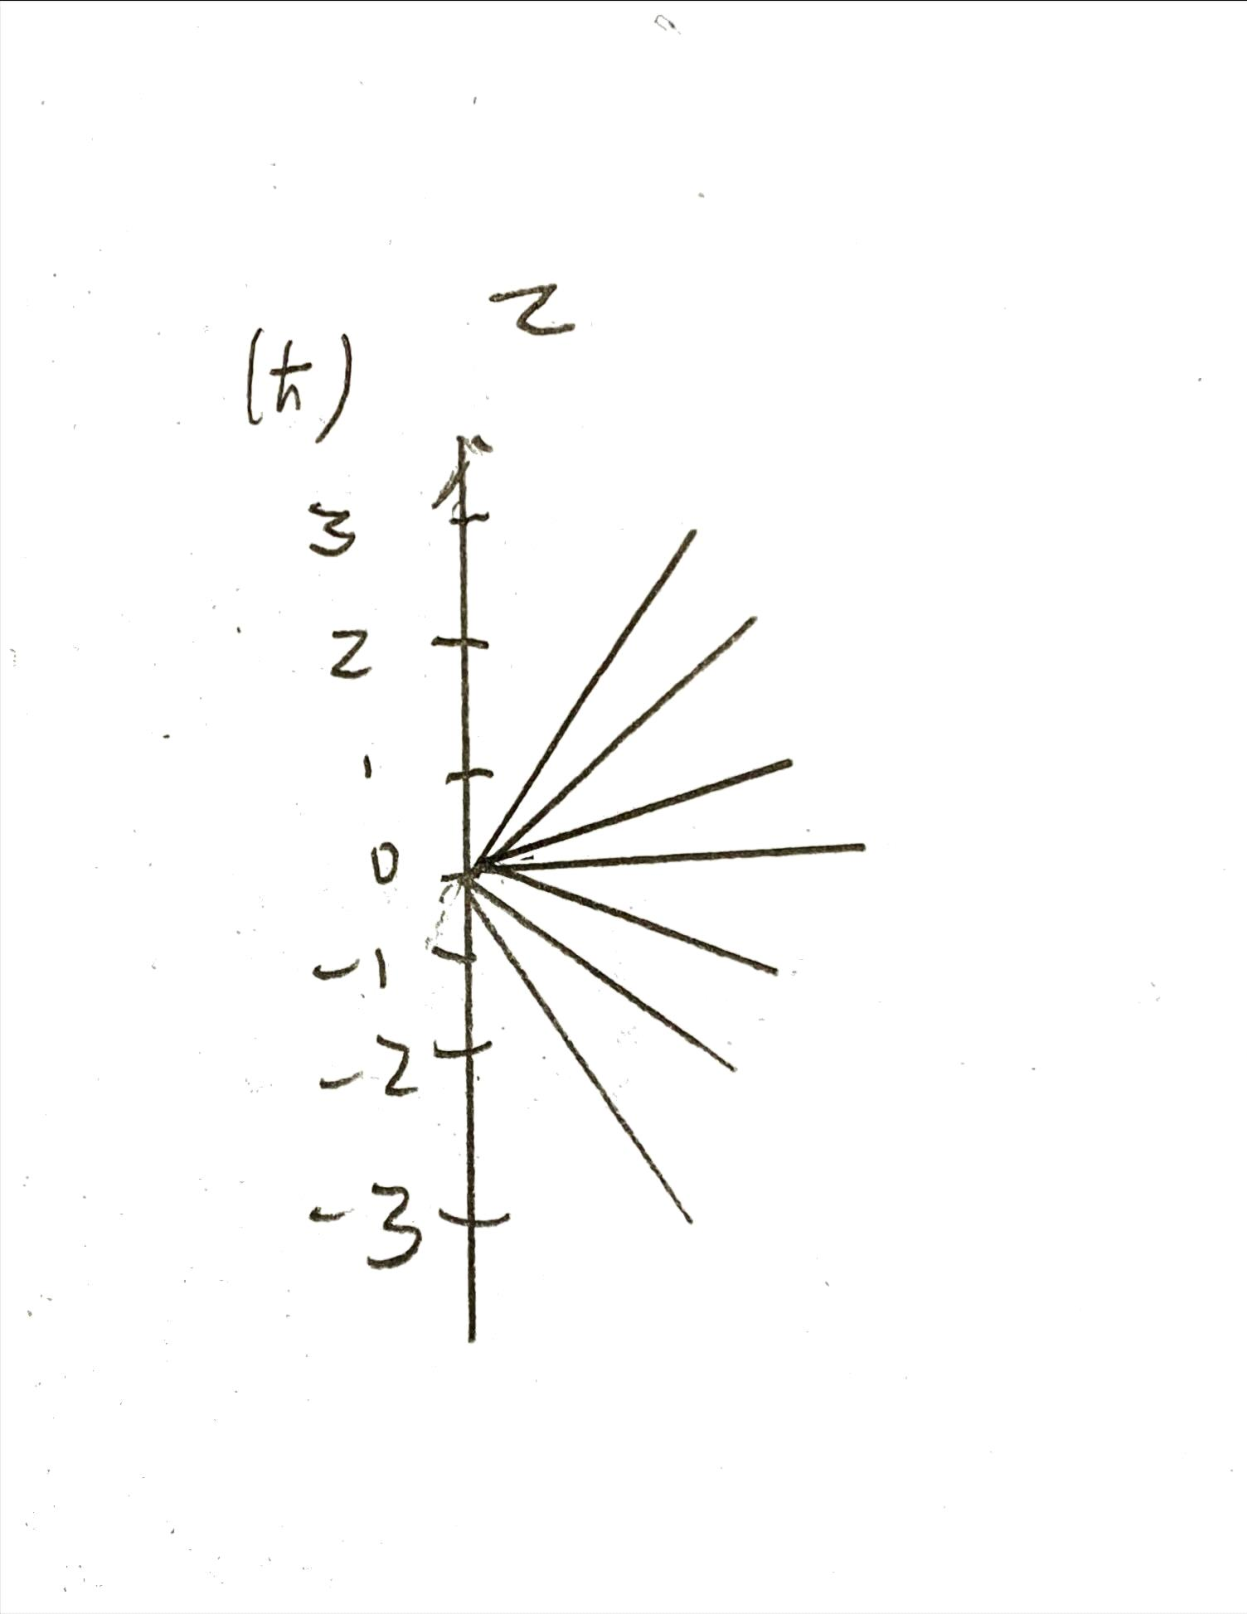
\includegraphics[width=0.7\textwidth]{Fizz.pdf}
\end{solution}

\question{The allowed magnitudes of the angular momentum are $L = \sqrt{l(l+1)\hbar}$ of $\vec{L}$, whereas the Bohr model assumes that $L=l\hbar$. Compute the ratio L(correct)/L(Bohr) for $l=1,2,3,4,10$, and $100$. Comment.}

\begin{solution}
	$$\sqrt{2}, \frac{\sqrt{6}}{2}, \frac{2\sqrt{3}}{3}, \frac{\sqrt{5}}{2}, \frac{\sqrt{110}}{10}, \frac{\sqrt{10100}}{100}$$
	or
	$$1.414,1.225,1.155,1.118,1.049, 1.005$$
	It (obviously) tends to 1, so Bohr's model becomes more and more accurate as $l$ increases.
\end{solution}

\question{The mean value (or expectation value) of $\frac{1}{r}$ for any state is $\langle\frac{1}{r}\rangle = \int_0^\infty \frac{1}{r}P(r)dr$. Find $\langle\frac{1}{r}\rangle$ for the $1s$ state of hydrogen. Comment.}

\begin{solution}
	$$P(r) = \frac{4}{a_B^3}r^2e^{-2r/a_B}$$
	The integral is then
	\begin{align*}
		I &= \frac{4}{a^3_B}\int_0^\infty re^{-2r/a_B} \\
		  &= \frac{4}{a^3_B}\left[-\frac{a_B}{2}re^{-2r/a_B} - e^{-2r/a_B}\times\frac{a^2_B}{4}\right]_0^\infty \\
		  &= \frac{4}{a^3_B}\times\frac{a^2_B}{4} \\
		  &= \frac{1}{a_B}
	\end{align*}
\end{solution}

\question{Use integration by parts to evaluate the integral in
	$$4\pi A^2\int_0^\infty r^2e^{-2r/a_B}dr=1$$
and hence verify that the normalization constant for the $1s$ wave function is $A = \frac{1}{\sqrt{\pi a^3_B}}$.}

\begin{solution}
	\begin{align*}
		I &= -\frac{a_B}{2}r^2e^{-2r/a_B} \Big |_0^\infty + a_B\int_0^\infty re^{-2r/a_B}dr \\
		  &= a_B\left[-\frac{a_B}{2}re^{-2r/a_B} - e^{-2r/a_B}\times\frac{a^2_B}{4}\right]_0^\infty \\
		  &= \frac{a^3_B}{4}
	\end{align*}
\end{solution}

\question{The average (or expectation) value $\langle r\rangle$ of the radius for any state is $\int_0^\infty rP(r)dr$. Find $\langle r\rangle$ for the $1s$ state of hydrogen. Explain the difference between the average and most probable radii.}

\begin{solution}
	The desired integral is
	$$\frac{4}{a^3_B}\int_0^\infty r^3e^{-2r/a_B}dr$$
	Using integral by parts, the first term obviously goes to zero at infinity, because of the exponential term, and at zero, because of the $r^3$ term. Therefore, this simplifies to
	$$\frac{6}{a^2_B}\int_0^\infty r^2e^{-2r/a_B}dr$$
	Similarly, this can be integrated to be
	$$\frac{6}{a_B}\int_0^\infty re^{-2r/a_B}dr$$
	and then
	$$3\int_0^\infty e^{-2r/a_B}dr$$
	which gives
	$$\frac{3a_B}{2}$$
	The average radius is the radius weighted by the probabilities of all probable radii. The most probably radius is simply the maximum radius, and does not take into acccount probability distribution.
\end{solution}

\question{The probability of finding the electron in the region $r>a$ is $\int_a^\infty P(r)dr$. What is the probability that a $1s$ electron in hydrogen would be found outside the Bohr radius ($r>a_B$)?}

\begin{solution}
	\begin{align*}
		\frac{4}{a^3_B}\int_{a_B}^\infty r^2e^{-2r/a_B} &= -\frac{2}{a^2_B}r^2e^{-2r/a_B} \Big |_{a_B}^\infty + \frac{4}{a^2_B}\int_{a_B}^\infty re^{-2r/a_B}dr \\
								&= 2e^{-2} - \frac{2}{a_B}re^{-2r/a_B} \Big |_{a_B}^\infty + \frac{2}{a_B}\int_{a_B}^\infty e^{-2r/a_B}dr \\
								&= 2e^{-2} + 2e^{-2} - e^{-2r/a_B} \Big |_{a_B}^\infty \\
								&= 4e^{-2} + e^{-2} \\
								&= 5e^{-2}
	\end{align*}
\end{solution}

\question{}

\begin{parts}
	\part{Write down the $\theta$ equation for the $2p$ states with $m=\pm1$. Show that the solution in $\Theta(\theta) = \sin\theta$. This means the complete wave functions for the $2p$ states with $m=\pm1$ are
		$$\psi_{2,1,\pm1} = R_{2p}(r)\sin\theta e^{\pm i\phi}$$
	}

	\begin{solution}
		$$\frac{1}{\sin\theta}\frac{d}{d\theta}\left(\sin\theta\frac{d\Theta}{d\theta}\right) + \left(l(l+1) - \frac{m^2}{\sin^2\theta}\right)\Theta = 0$$
		The only possible value $l$ can take is $1$. Substituting,
		$$\frac{1}{\sin\theta}\frac{d}{d\theta}\left(\sin\theta\frac{d\Theta}{d\theta}\right) + \left(2 - \frac{1}{\sin^2\theta}\right)\Theta = 0$$
		Plugging in the answer, the left-hand side yields
		\begin{align*}
			\frac{1}{\sin\theta}\frac{d}{d\theta}(\sin\theta\cos\theta) + 2\sin\theta - \frac{1}{\sin\theta} &= \frac{\cos^2\theta}{\sin\theta} - \sin\theta + 2\sin\theta - \frac{1}{\sin\theta} \\
															 &= -\sin\theta - \sin\theta + 2\sin\theta \\
															 &= 0
		\end{align*}
	\end{solution}

	\part{Prove that the sum of these two wave functions is the $2p_x$ wave function (times an uninteresting factor of 2) and that the difference is the $2p_y$ function (times 2i).}

	\begin{solution}
		The sum is
		\begin{align*}
			R_{2p}(r)\sin\theta e^{i\phi} + R_{2p}(r)\sin\theta e^{-i\phi} &= R_{2p}(r)\sin\theta(\cos\phi + i\sin\phi + \cos\phi - i\sin\phi) \\
										       &= 2R_{2p}\sin\theta\cos\phi \\
										       &= 2x
		\end{align*}
		Where the last equality is the representation of $x$ in spherical coordinates. Similarly,
		\begin{align*}
			R_{2p}(r)\sin\theta e^{i\phi} - R_{2p}(r)\sin\theta e^{-i\phi} &= R_{2p}(r)\sin\theta(\cos\phi + i\sin\phi - \cos\phi + i\sin\phi) \\
										       &= 2iR_{2p}(r)\sin\theta\sin\phi \\
										       &= 2iy
		\end{align*}
		Where the last equality is the representation of $y$ in spherical coordinates.
	\end{solution}
\end{parts}

\question{Using the wave function, write down the radial probability density for a hydrogen atom in a state with $l = n-1$. Find the most probable radius. Notice that in this case the quantum mechanical answer agrees with the Bohr model.}

\begin{solution}
	$$R(r) = Ar^{n-1}e^{-r/a_B} = Ae^{-r/a_B}$$
	when substituting $n=1$ for hydrogen. The radial probability density is hence
	$$4\pi r^2|R(r)|^2 = 4A^2\pi r^2e^{-2r/a_B}$$
	Setting its derivative to 0,
	\begin{align*}
		8A^2\pi re^{-2r/a_B} - \frac{8}{a_B}A^2\pi r^2e^{-2r/a_B} &= 0 \\
		1 - \frac{r}{a_B} &= 0 \\
		r &= a_B
	\end{align*}
	which is the radius given by the Bohr model.
\end{solution}

\question{Write down the radial density $P(r)$ for the $2s$ and $2p$ states of hydrogen. Find the most probable radius for each of these states.}

\begin{solution}
	$$P_{2s}(r) = 4\pi r^2 A^2\left(2-\frac{r}{a_B}\right)^2 e^{-r/a_B}$$
	$$P_{2p}(r) = 4\pi A^2r^4e^{-r/a_B}$$
	Ignoring the constants and taking the square root, we maximize for $2s$.
	\begin{align*}
		\left(2-\frac{r}{a_B}\right)e^{-r/2a_B} - \frac{r}{a_B} e^{-r/2a_B} - \frac{r}{2a_B}\left(2-\frac{r}{a_B}\right) e^{-r/2a_B} &= 0 \\
		2-\frac{r}{a_B} - \frac{r}{a_B} - \frac{r}{a_B} + \frac{r^2}{2a^2_B} &= 0 \\
		2 - \frac{3r}{a_B} + \frac{r^2}{2a^2_B} &= 0 \\
		r &= (3+\sqrt{13})a_B
	\end{align*}
	where (obviously) only the positive root is taken. Similarly, but without taking the square root,
	\begin{align*}
		4r^3e^{-r/a_B} - \frac{r^4}{a_B}e^{-r/a_B} &= 0 \\
		4 - \frac{r}{a_B} &= 0 \\
		r &= 4a_B
	\end{align*}
\end{solution}

\question{What is the most probable radius for a $1s$ electron in the hydrogen-like ion Ni$^{27+}$? What is its binding energy?}

\begin{solution}
	For hydrogen-like ions, radius is pulled inwards by a factor of the charge, so the most probable radius is $\frac{a_B}{28}$. Similarly, energy is scaled by $Z^2$, giving
	$$13.6 \times 28^2 = 10.7\unit{k.eV}$$
\end{solution}
\end{questions}
\end{document}
